\section{Geometry of $\mathbb{R}^n$}

Each vector $\begin{bmatrix}v_1\\v_2 \\ \vdots \\ v_n \end{bmatrix} \in \mathbb{R}^n$ can be visualized as an arrow going from the origin 
$(0,0, \ldots, 0)$ to the point $(v_1, v_2, \ldots, v_n)$.  In this case we'd call the \textbf{base point} the origin.

\begin{example}
$\begin{bmatrix}2\\5\end{bmatrix}$ can be visualized as the arrow between $(0,0)$ and $(2,5)$\\
\begin{center}
  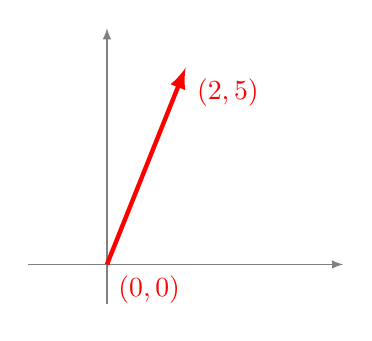
\begin{tikzpicture}[scale=.5]
    \coordinate (Origin)   at (0,0);
    \coordinate (XAxisMin) at (-2,0);
    \coordinate (XAxisMax) at (6,0);
    \coordinate (YAxisMin) at (0,-1);
    \coordinate (YAxisMax) at (0,6);
    \draw [thin, gray,-latex] (XAxisMin) -- (XAxisMax);% Draw x axis
    \draw [thin, gray,-latex] (YAxisMin) -- (YAxisMax);% Draw y axis
    \draw [ultra thick,-latex,red] (Origin) node [below right] {$(0,0)$} -- (2,5) node [below right] {$(2,5)$};
  \end{tikzpicture}
\end{center}
\end{example}

We can also think of any arrow from point $(a_1, a_2, \ldots, a_n)$ to point $(b_1, b_2, \ldots, b_n)$ as a vector. We've simply changed 
the \text{base point} to $(a_1, a_2, \ldots, a_n)$ instead of the origin. 

\begin{definition}
The \textbf{canonical form} of a vector from $(a_1, a_2, \ldots, a_n)$ to $(b_1, b_2, \ldots, b_n)$ is the vector 
$\begin{bmatrix}b_1-a_1 \\ b_2-a_2 \\ \vdots \\ b_n-a_n\end{bmatrix}$
\end{definition}

\begin{remark}
You can think of the canonical form of a vector is taking an arrow with the same length and direction with base point of the origin.
\end{remark}

\begin{example}
The vector from $(2,3)$ to $(3,-2)$ has canonical form $\begin{bmatrix*}[C]1\\-5\end{bmatrix*}$. Below the vector is in red and the canonical form of the vector is in blue.\\
\begin{center}
  \begin{tikzpicture}[scale=.5]
    \coordinate (Origin)   at (0,0);
    \coordinate (XAxisMin) at (-6,0);
    \coordinate (XAxisMax) at (6,0);
    \coordinate (YAxisMin) at (0,-6);
    \coordinate (YAxisMax) at (0,6);
    \draw [thin, gray,-latex] (XAxisMin) -- (XAxisMax);% Draw x axis                                                                                                   
    \draw [thin, gray,-latex] (YAxisMin) -- (YAxisMax);% Draw y axis                                                                                                   
    \draw [ultra thick,-latex,red] (2,3) node [above right] {$(2,3)$} -- (3,-2) node [above right] {$(3,-2)$};
    \draw [ultra thick,-latex,blue] (Origin) node [above right] {$(0,0)$} -- (1,-5) node [above right] {$(3,-2)$};
  \end{tikzpicture}
  \end{center}
\end{example}

\subsection{Scalar Multiplication and Vector Addition}

Scalar multiplication can be thought of as a  geometric operation. If $r>0$ then $r\vec{v}$ can be thought of as $v$ stretched or shrunk by real factor $r$.\\ 
\begin{center}
\begin{tikzpicture}[scale=.5]
    \coordinate (Origin)   at (0,0);
    \coordinate (XAxisMin) at (-6,0);
    \coordinate (XAxisMax) at (6,0);
    \coordinate (YAxisMin) at (0,-6);
    \coordinate (YAxisMax) at (0,6);
    \draw [thin, gray,-latex] (XAxisMin) -- (XAxisMax);% Draw x axis                                                                                                   
    \draw [thin, gray,-latex] (YAxisMin) -- (YAxisMax);% Draw y axis                                                                                                   
    \draw [ultra thick,-latex,blue] (0,0)  -- (6,3) node[pos=0.5,above]{$r\vec{v}$};
    \draw [ultra thick,-latex,black] (Origin) -- (2,1) node[pos=0.5,above]{$\vec{v}$};;
\end{tikzpicture}
\end{center}
If $r<0$ then $r\vec{v}$ can be thought of as $v$ reflected through the origin then stretced or shrunk by a real factor $|r|$
\begin{center}
\begin{tikzpicture}[scale=.5]
    \coordinate (Origin)   at (0,0);
    \coordinate (XAxisMin) at (-6,0);
    \coordinate (XAxisMax) at (6,0);
    \coordinate (YAxisMin) at (0,-6);
    \coordinate (YAxisMax) at (0,6);
    \draw [thin, gray,-latex] (XAxisMin) -- (XAxisMax);% Draw x axis                                                                                                   
    \draw [thin, gray,-latex] (YAxisMin) -- (YAxisMax);% Draw y axis                                                                                                   
    \draw [ultra thick,-latex,blue] (0,0)  -- (-6,-3) node[pos=0.5,above]{$r\vec{v}$};
    \draw [ultra thick,-latex,black] (Origin) -- (2,1) node[pos=0.5,above]{$\vec{v}$};;
\end{tikzpicture}
\end{center}
Vector addition can also be thought of as a geometric operation via the \textbf{parallelogram rule}. 

\begin{proposition}[The Paralelogram Rule] If $\vec{v},\vec{w} \in \mathbb{R}^n$ with then $\vec{v}+\vec{w}$ can be determined by the following:
\begin{enumerate}
\item If there is a nonzero linear combination $s\vec{v}+t\vec{w}$ equal to $\vec{0}$ then 
$\vec{v}+\vec{w}$ is either a scalar multiple of $\vec{v}$ or a scalar multiple of $\vec{w}$.

\item Otherwise $\vec{v}+\vec{w}$ is determined by the parallelogram rule:\\
\begin{center}
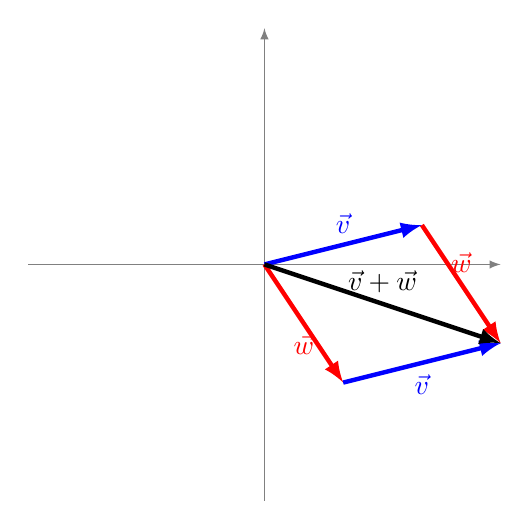
\begin{tikzpicture}[scale=.5]
    \coordinate (Origin)   at (0,0);
    \coordinate (XAxisMin) at (-6,0);
    \coordinate (XAxisMax) at (6,0);
    \coordinate (YAxisMin) at (0,-6);
    \coordinate (YAxisMax) at (0,6);
    \draw [thin, gray,-latex] (XAxisMin) -- (XAxisMax);% Draw x axis                                                                                                   
    \draw [thin, gray,-latex] (YAxisMin) -- (YAxisMax);% Draw y axis                                                                                                   
    \draw [ultra thick,-latex,blue] (0,0)  -- (4,1) node[pos=0.5,above]{$\vec{v}$};
    \draw [ultra thick,-latex,red] (4,1)  -- (6,-2) node[pos=0.5,above]{$\vec{w}$};
    \draw [ultra thick,-latex,red] (Origin) -- (2,-3) node[pos=0.5,below]{$\vec{w}$};;
    \draw [ultra thick,-latex,blue] (2,-3)  -- (6,-2) node[pos=0.5,below]{$\vec{v}$};
    \draw [ultra thick,-latex,black] (0,0)  -- (6,-2) node[pos=0.5,above]{$\vec{v}+\vec{w}$};
\end{tikzpicture}
\end{center}
Note that taking the base point of $\vec{w}$ to be the end point of $\vec{v}$ yeilds the same result as taking the base point of $\vec{v}$ to be the end point of 
$\vec{w}$.
\end{enumerate}
\end{proposition}
\begin{proof}
The proof of the case where there is a nonzero linear combination of $s\vec{v}+t\vec{w}=\vec{0}$ is Exercise~\ref{exercise:dependent_addition}. This case eliminates the possiblity that $\vec{v}$ and $\vec{w}$ are on the same line.

The vector $\vec{v}$ take the origin $(0,0, \ldots, 0)$ to the coordinate $(v_1, v_2, \ldots, v_n)$. 
By adding vector $w$ we take $(v_1, v_2, \ldots, v_n)$ to $(v_1+w_1, v_2+w_2, \ldots, v_n+w_n)$. 
So $v+w$ is the composite operation of taking the origin to $(v_1, v_2, \ldots, v_n)$ then to $(v_1+w_1, v_2+w_2, \ldots, v_n+w_n)$. 

Graphically we can think of this as follow the canonical form of $\vec{v}$ then base $w$ at the endpoint of $v$ to get $\vec{v}+\vec{w}$. Since we can do the same thing starting with $w$, this makes a parallelogram as long as $\vec{v}$ and $\vec{w}$ are not on the same line.
\end{proof}

\begin{example} 
Let $\vec{v}=\begin{bmatrix} 1 \\ 3 \end{bmatrix}$ and $\vec{w}=\begin{bmatrix*}[C] -5 \\ 2 \end{bmatrix*}$. We can identify all vectors in $\mathbb{R}^n$ as a linear combination of these two geometrically. Since the canonical forms of$\vec{v}$ and $\vec{w}$ are not in the same line in $\mathbb{R}^n$, $\vec{v}+\vec{w}$ forms a parallelogram. Below we mark all the integer linear combination endpoints of $m\vec{v}+n\vec{w}$ where $n$ and $m$ are integers. This makes a shape called a lattice:
\begin{center}
\includegraphics[scale=.5]{Rn/vw_graph1.pdf}
\end{center}

We can see below that the vector $\begin{bmatrix*}[C]9 \\ -7 \end{bmatrix*}$ can be written by the linear combination $(-1)\vec{v}+(-2)\vec{w}$. It doesn't even mater what path we use to get there since we can use the associative properties of vector addition and the distributive property of vector addition and scalar multiplication.
\begin{center}
\includegraphics[scale=.5]{Rn/vw_9n7_graph1.pdf}
\end{center}

It's not a very large stretch to include vectors with endpoints on the rest of the plane since all we need to allow is any real linear combination $r\vec{v}+t\vec{w}$ where $r$ and $t$ are real numbers. For instance we can add in the endpoint $(3,3)$ by taking $\frac{21}{17}\vec{v}+\frac{-6}{17}\vec{w}$\\
\begin{center}
\includegraphics[scale=.5]{Rn/vw_graph2.pdf}\
\end{center}
\end{example}
\begin{remark}
The above example illustrates that you can build a whole plane with linear combinations of two vectors.
\end{remark}
\begin{definition}[The Span]
We call the set of linear combinations of a collection of vectors in $\mathbb{R}^n$ the \textbf{span}.
\[
\text{span}\{ \vec{v}_1, \vec{v}_2, \ldots, \vec{v}_k \}=
\{a_1\vec{v}_1+a_2\vec{v}_2+\cdots+a_k\vec{v}_k \mid a_1, a_2, \ldots , a_k \in \mathbb{R} \}
\]
\end{definition}

\begin{example} Consider the following span
\[
H=\text{span}\left\{
\begin{bmatrix*}[C]1 \\ 0 \\ 0 \\ -1\end{bmatrix*},
\begin{bmatrix*}[C]-1 \\ 2 \\ 1 \\ 0\end{bmatrix*},
\begin{bmatrix*}[C]0 \\ 1 \\ 1 \\ 1\end{bmatrix*}
\right\}
\]

Each $\vec{v} \in H$ can be written as a liner combination:
\[
\vec{v}=
x_1\begin{bmatrix*}[C]1 \\ 0 \\ 0 \\ -1\end{bmatrix*}+
x_2\begin{bmatrix*}[C]-1 \\ 2 \\ 1 \\ 0\end{bmatrix*}+
x_3\begin{bmatrix*}[C]0 \\ 1 \\ 1 \\ 1\end{bmatrix*}
\]
for some choice of $x_1, x_2, x_3 \in \mathbb{R}$. This in turn can be written
as matrix vector multiplication:
\[
\vec{v}=
x_1\begin{bmatrix*}[C]1 \\ 0 \\ 0 \\ -1\end{bmatrix*}+
x_2\begin{bmatrix*}[C]-1 \\ 2 \\ 1 \\ 0\end{bmatrix*}+
x_3\begin{bmatrix*}[C]0 \\ 1 \\ 1 \\ 1\end{bmatrix*}
=
\begin{bmatrix*}[C]
1 & -1 & 0 \\
0 & 2 & 1 \\
0 & 1 & 1 \\
-1 & 0 & 1 
\end{bmatrix*}
\begin{bmatrix}
x_1 \\ x_2 \\ x_3
\end{bmatrix}
\]

So the linear transformation $T:\mathbb{R}^3 \to \mathbb{R}^4$ defined by 
\[
T(\vec{x})=\begin{bmatrix*}[C]
1 & -1 & 0 \\
0 & 2 & 1 \\
0 & 1 & 1 \\
-1 & 0 & 1 
\end{bmatrix*}
\begin{bmatrix}x_1 \\ x_2 \\ x_3 \end{bmatrix}
\]
takes coordinates on each of the vectors to the appropriate linear combination in $H$.
\end{example}
\begin{example} We can describe the image of a linear transformation using a span quite easily. For example $T:\mathbb{R}^3 \to \mathbb{R}^5$ defined by
\[
T(\vec{v})=\begin{bmatrix*}[C]
1 & 0 & -1 \\
0 & -1 & 5 \\
2 & 0 & 0 \\
-3 & 3 & 3 \\
3 & 3 & -2 \\
\end{bmatrix*}\begin{bmatrix}v_1\\ v_2\\ v_3\end{bmatrix}
=
v_ 1\begin{bmatrix*}[C]1 \\ 0 \\ 2 \\ -3 \\ 3 \end{bmatrix*}
+v_2\begin{bmatrix*}[C]0 \\ -1 \\ 0 \\ 3 \\ 3 \end{bmatrix*}
+v_3\begin{bmatrix*}[C]-1 \\ 5 \\ 0 \\ 3 \\ 2 \end{bmatrix*}
\] 

So we can rewrite the image of $T$ as 

\[
\text{span}\left\{
\begin{bmatrix*}[C]1 \\ 0 \\ 2 \\ -3 \\ 3 \end{bmatrix*},
\begin{bmatrix*}[C]0 \\ -1 \\ 0 \\ 3 \\ 3 \end{bmatrix*},
\begin{bmatrix*}[C]-1 \\ 5 \\ 0 \\ 3 \\ 2 \end{bmatrix*}
\right\}
=\left\{
v_ 1\begin{bmatrix*}[C]1 \\ 0 \\ 2 \\ -3 \\ 3 \end{bmatrix*}
+v_2\begin{bmatrix*}[C]0 \\ -1 \\ 0 \\ 3 \\ 3 \end{bmatrix*}
+v_3\begin{bmatrix*}[C]-1 \\ 5 \\ 0 \\ 3 \\ 2 \end{bmatrix*}
\mid 
v_1, v_2, v_3 \in \mathbb{R}^5 
\right\}
\]
\end{example}
\subsubsection{Exercises}

\begin{exercise} Find the canonical form of each of the following vectors:\\
\begin{inparaenum}[a)]
\item a vector from $(0,0)$ to $(1,3)$ in $\mathbb{R}^2$\\
\item a vector from $(1,2)$ to $(5,6)$ in $\mathbb{R}^2$\\
\item a vector from $(0,0,1)$ to $(-3,1,5)$ in $\mathbb{R}^3$\\
\item a vector from $(3,0,-2)$ to $(0,0,0)$ in $\mathbb{R}^3$\\
\end{inparaenum}
\end{exercise}

\begin{exercise} Draw a lattice of enpoints of vectors $\vec{u}=\begin{bmatrix}2\\1\end{bmatrix}$ and $\vec{v}=\begin{bmatrix}1\\-5\end{bmatrix}$. That is graph 
$m\vec{u}+n\vec{v}$ for integer values of $m$ and $n$. Use the lattice to graphically determine, or estimate, the coefficients $r$ and $t$ for the linear combination of $r\vec{u}+t\vec{v}$ that gives the vector below:\\
\begin{inparaenum}
\item $\begin{bmatrix}3 \\ 7 \end{bmatrix}$\hfill 
\item $\begin{bmatrix*}[C]-1 \\ -6 \end{bmatrix*}$\hfill {} \\
\item $\begin{bmatrix*}[C]-9 \\ 1 \end{bmatrix*}$\hfill 
\item $\begin{bmatrix*}[C] 0 \\ -5.5 \end{bmatrix*}$\hfill {} \\
\end{inparaenum}
\end{exercise}



\subsection{Linear Dependence and Linear Independence}

Previously, we noticed that when we add two vectors $\vec{v}+\vec{w}$, the result can geometrically be described either by linear addition or by the parallelogram rule. When the result is linear addition the vectors are on the same line in $\mathbb{R}^n$. In other words $\vec{v}=r\vec{w}$ or $\vec{w}=t\vec{v}$ for some $r,t \in \mathbb{R}$. Instead of stating this as two cases, we can instead write 

\begin{equation*}
a\vec{v}+b\vec{w}=\vec{0}
\end{equation*}

where $a$ and $b$ are real scalars and they are not both zero. We call the case where both $a=0$ and $b=0$ the \textbf{trivial solution} to the vector equation and any solution where at least one of them is non-zero a \textbf{non-trivial solution}.

Generalizing to more than two vectors we get the following definition:

\begin{definition}[Linearly Dependent Vectors]
Vectors $\vec{v}_1, \vec{v}_2, \ldots, \vec{v}_n \in \mathbb{R}^m$ are \textbf{linearly dependent} if 

$$x_1\vec{v}_1+x_2\vec{v}_2+\cdots + x_n \vec{v}_n=\vec{0}$$

has a \textbf{non-trivial solution}. That is, there is a solution $x_1, x_2, \ldots, x_n$ to the vector equation with $x_i \neq 0$ for at least one value $i$. 
\end{definition}

\begin{proposition} Vectors $\vec{v}_1, \vec{v}_2, \ldots, \vec{v}_n \in \mathbb{R}^n$ are linearly dependent if and only if at at least one of the vectors, $\vec{v}_k$, can be written as a linear combination of the others. That is,
$$
\vec{v}_k=\alpha_1 v_1+ \cdots+ \alpha_{k-1}\vec{v}_{k-1}+ \alpha_{k+1}\vec{v}_{k+1}+\cdots+ \alpha_n \vec{v}_n
$$
\end{proposition}
\begin{proof}
Let $\vec{v}_1, \vec{v}_2, \ldots, \vec{v}_n \in \mathbb{R}^n$ be linearly dependent. Then there is a nontrivial solution to:

$$x_1\vec{v}_1+x_2\vec{v}_2+\cdots +x_{k-1}\vec{v}_{k-1}+ x_k\vec{v}_k+x_{k+1}\vec{v}_{k+1}+ \cdots + x_n \vec{v}_n=\vec{0}$$

That is $x_k \neq 0$ for some $k$. Solving for $x_k\vec{v}_k$ we get

$$
(-x_k)\vec{v}_k=x_1 v_1+ \cdots + x_{k-1}\vec{v}_{k-1}+ x_{k+1}\vec{v}_{k+1}+\cdots+ x_n \vec{v}_n
$$

Since $x_k \neq 0$ we can multiply both sides of the equation by $-\frac{1}{x_k}$ yeilding:

$$
\vec{v}_k=\frac{x_1}{-x_k} v_1+ \cdots + \frac{x_{k-1}}{-x_k}\vec{v}_{k-1}+ \frac{x_{k+1}}{-x_k}\vec{v}_{k+1}+\cdots+ \frac{x_n}{-x_k} \vec{v}_n
$$

To show the converse let 

$$\vec{v}_k=\alpha_1 v_1+ \cdots+ \alpha_{k-1}\vec{v}_{k-1}+ \alpha_{k+1}\vec{v}_{k+1}+\cdots+ \alpha_n \vec{v}_n$$

Then by adding $(-1)\vec{v}_k$ to both sides
$$
\vec{0}=\alpha_1 v_1+ \cdots+ \alpha_{k-1}\vec{v}_{k-1}+(-1)\vec{v}_k+ \alpha_{k+1}\vec{v}_{k+1}+\cdots+ \alpha_n \vec{v}_n
$$

This is a non-trivial linear combination of $\vec{v}_1, \vec{v}_2, \ldots, \vec{v}_k$ since the $k$-coefficient $(-1)$ is nonzero. Therefore, $\vec{v}_1, \vec{v}_2, \ldots, \vec{v}_k$ are linearly dependent.
\end{proof}

\begin{remark}
The above proposition shows that a linearly dependent set has ``extra vectors'' when it comes to making linear combinations. That is, by adding in a vector $\vec{v}_k$, that can be written as a linear combination of the others you could have accomplished the same thing by simply changing the coefficients on the other vectors. So in a sense the $\vec{v}_k$ vector is unnecessary or ``extra'' and there could be more than one such vector.
\end{remark}

\begin{proposition}\label{prop:zero_dependent} If the zero vector is in a set of vectors then the set is linearly dependent. 
\end{proposition}
\begin{proof}
Left as an exercise.
\end{proof}


\begin{proposition}\label{prop:zero_dependent} If the row vectors of matrix $A \in M_{m\times n}(\mathbb{R})$ are linearly dependent, then there is a  $\vec{b} \in \mathbb{R}^m$ such that $A\vec{v}=\vec{b}$ does not have a solution.
\end{proposition}
\begin{proof}
Let $A$ have row vectors $\vec{r}_1, \vec{r}_2, \ldots, \vec{r}_m$ in $\mathbb{R}^n_\text{row}$ and suppose they are linearly dependent. Then for some $k$ a row vector
$\vec{r}_k$ is a linear combination of the other row vectors. That is,
\[
\vec{r}_k=a_1\vec{r}_1+\cdots+a_{k-1}\vec{r}_{k-1}+a_{k+1}\vec{r}_{k+1}+\cdots+a_m\vec{r}_m
\]

Thus when we set $A\vec{v}=\vec{b}$ we get 
\begin{align*}
A\vec{v} = \begin{bmatrix}\vec{r}_1 \\ \vec{r}_2 \\ \vdots \\ \vec{r}_k \\ \vdots \\ \vec{r}_m\end{bmatrix}\vec{v}
= \begin{bmatrix}\vec{r}_1\vec{v} \\ \vec{r}_2\vec{v} \\ \vdots \\ \vec{r}_k\vec{v} \\ \vdots \\ \vec{r}_m\vec{v}\end{bmatrix}
=\begin{bmatrix}b_1 \\ b_2 \\ \vdots \\ b_k \\ \vdots \\ b_m\end{bmatrix}
\end{align*}

If we set $b_i=0$ for all $i \neq k$ and $b_k=1$ we then have a $\vec{b}$ such that $A\vec{v}=\vec{b}$ has no solution. If $\vec{v}$ were a solution  
then $\vec{r}_i\vec{v}=0$  for all $i \neq k$ and $\vec{r}_k\vec{v}=1$, but 
\begin{align*}
\vec{r}_k\vec{v} &= (a_1\vec{r}_1+\cdots+a_{k-1}\vec{r}_{k-1}+a_{k+1}\vec{r}_{k+1}+\cdots+a_m\vec{r}_m)\vec{v}\\
&= a_1\vec{r}_1\vec{v}+\cdots+a_{k-1}\vec{r}_{k-1}\vec{v}+a_{k+1}\vec{r}_{k+1}\vec{v}+\cdots+a_m\vec{r}_m\vec{v}\\
&= a_10+\cdots+a_{k-1}0+a_{k+1}0+\cdots+a_m0\\
&= 0
\end{align*}
\end{proof}

\begin{proposition}\label{prop:zero_dependent} If the column vectors of matrix $[\vec{a}_1, \ldots, \vec{a}_n]=A \in M_{m\times n}(\mathbb{R})$ are linearly dependent and $\vec{w}$ is a solution to $A\vec{v}=\vec{b}$ then there are infinitely many solutions to $A\vec{v}=\vec{b}$.
\end{proposition}
\begin{proof}
Left as an exercise.
\end{proof}

\begin{definition}[Linearly Independent Vectors]
Vectors $\vec{v}_1, \vec{v}_2, \ldots, \vec{v}_n \in \mathbb{R}^m$ are \textbf{linearly independent} if 

$$x_1\vec{v}_1+x_2\vec{v}_2+\cdots + x_n \vec{v}_n=\vec{0}$$

has only the \textbf{trivial solution}. That is, the only solution to the vector equation is $x_1=x_2=\cdots=x_n=0$.  
\end{definition}

\subsection{Geometric Transformations}

\subsection{Dot Product, Distance and Angle between vectors}

